%%
%% This is file `sample-sigconf-authordraft.tex',
%% generated with the docstrip utility.
%%
%% The original source files were:
%%
%% samples.dtx  (with options: `all,proceedings,bibtex,authordraft')
%% 


\documentclass[sigconf]{acmart}

\usepackage{listings}
\usepackage{xcolor}

\definecolor{codebg}{rgb}{0.95,0.95,0.95}
\definecolor{string}{rgb}{0.63,0.13,0.94}
\definecolor{keyword}{rgb}{0.13,0.13,1}

\lstset{
    backgroundcolor=\color{codebg},
    basicstyle=\ttfamily\small,
    keywordstyle=\color{keyword}\bfseries,
    stringstyle=\color{string},
    commentstyle=\color{gray},
    numbers=left,
    numberstyle=\tiny\color{gray},
    stepnumber=1,
    numbersep=10pt,
    showspaces=false,
    showstringspaces=false,
    showtabs=false,
    frame=single,
    tabsize=4,
    captionpos=b,
    breaklines=true,
    breakatwhitespace=false,
    escapeinside={\%*}{*)}
}


\begin{document}

%%
%% The "title" command has an optional parameter,
%% allowing the author to define a "short title" to be used in page headers.
\title{TabFill: Sketch-Guided Missing Value Imputation on Tabular Data via Large Language Models}


\author{Changlun Li}
\affiliation{%
  \institution{The Hong Kong University of Science and Technology (Guangzhou)}
  \city{Guangzhou City}
  \country{China}}
\email{cli942@connect.hkust-gz.edu.cn}


% \renewcommand{\shortauthors}{Trovato et al.}

%%
%% The abstract is a short summary of the work to be presented in the
%% article.
\begin{abstract}
Data preprocessing plays a pivotal role in data-driven analysis, with Missing Value Imputation (MVI) standing out as a crucial and time-consuming task. Despite extensive efforts devoted to MVI, existing approaches often fall short in accuracy, relying on simple methods such as descriptive statistics like mean, mode, or zero imputation. In this paper, we present TabFill, a novel approach to archive MVI through the power of Large Language Models (LLMs). TabFill brings up a combination strategy: sketch and code generation. Firstly, user can sketch a series of planning steps to guide LLM in providing answers with explanations. Later, those results would be constrained into a structured Python code via CodeLLM. This approach not only improves the reliability and efficiency of imputations but also facilitates human review by presenting clear, actionable code. Through empirical evaluations on diverse datasets, we demonstrate that TabFill significantly enhances MVI efficiency and maintain good accuracy, offering a promising advancement in data preprocessing techniques for data-driven analyses. We have released codes in Github: https://github.com/tigerlcl/llm-sketch.
\end{abstract}


\keywords{Data preparation, Missing value imputation, Large language model}


\maketitle


\section{Introduction}
In the era of data-driven decision-making, the quality of the data being analyzed is paramount. As the adage goes, "rubbish in, rubbish out." This highlights the importance of data preprocessing, particularly Missing Value Imputation (MVI), which ensures that machine learning models are fed with high-quality datasets. Without proper handling of missing data, the predictive ability of these models can be significantly compromised due to the contamination from incomplete records. Missing data is a ubiquitous problem across various domains, from healthcare to finance~\cite{andridge2010review,emmanuel2021survey}. Studies have shown that in real-world datasets, the prevalence of missing data can range from minor omissions to substantial portions of the dataset, often exceeding 30\% in certain cases~\cite{emmanuel2021survey}. This presents a substantial challenge, as inaccurate handling of these gaps can lead to biased and unreliable analytical outcomes. Existing MVI techniques come with several notable limitations:

\begin{itemize}
  \item Out-dated approach:
  Methods such as mean, mode, or hot-deck imputation~\cite{andridge2010review,little2019statistical} often lack the accuracy needed for high-quality data analysis, as shown in Figure~\ref{fig:method}(a). These techniques can still leave data in a dirty state or necessitate the removal of incomplete records. Besides, traditional methods fail to leverage the context provided by existing entries in the dataset or domain-specific knowledge, resulting in suboptimal imputation.
  \item Human-aided overhead:
  Data scientists reportedly spend up to 80\% of their project time on data cleaning tasks~\cite{emmanuel2021survey}, which includes MVI. This high level of manual effort is not scalable and can lead to inconsistencies and errors. The reliance on human intervention for imputing missing values is labor-intensive and time-consuming, diverting valuable resources away from more strategic analytical tasks.
\end{itemize}

\begin{figure}[h]
  \centering
  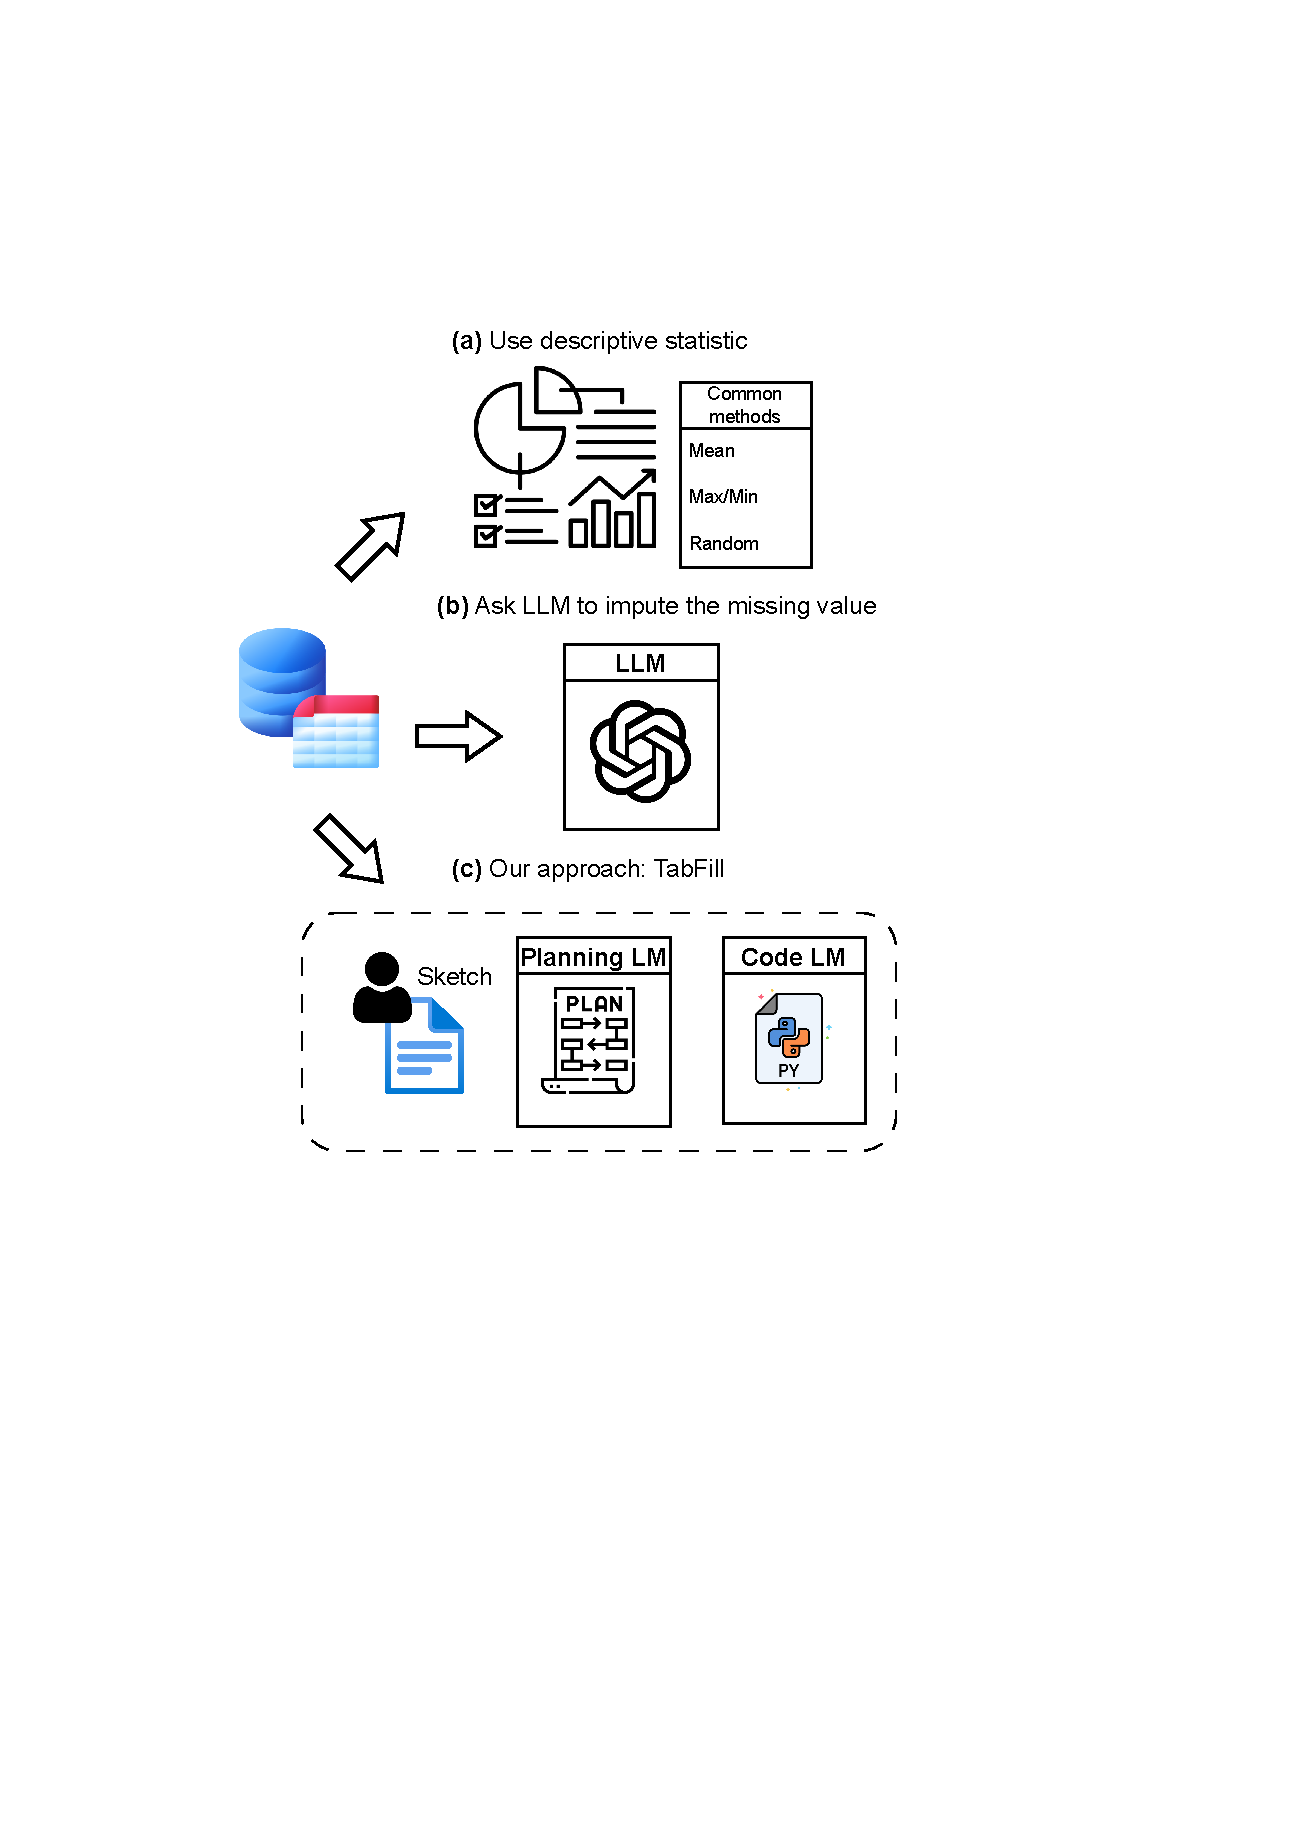
\includegraphics[width=0.7\linewidth]{methods.pdf}
  \caption{Imputation using different approaches}
  \label{fig:method}
\end{figure}

In recent years, large language models (LLMs) have shown considerable promise in addressing complex data processing tasks, thanks to their profound capabilities~\cite{zhao2023survey}, table understanding~\cite{sui2024table, zha2023tablegpt, li2023table} in knowledge extraction and content generation. Their ability to understand and manipulate textual and, increasingly, non-textual data suggests a promising avenue for enhancing MVI techniques. Therefore, we explored two existing LLM approaches: 1) instruct LLM directly to perform MVI on dirty data (see Figure~\ref{fig:method}(b)); 2) employ Chain-of-Thought prompting~\cite{wei2023chainofthought} to enhance their reasoning process on MVI. However, Challenges were revealed by the LLM output due to unreliable and extensive explanations. LLM exhibits insufficient filling rate when confronted with numerous missing values.

To address above challenges, we propose TabFill (see Figure~\ref{fig:method}(c)), a novel framework that combines sketch-based guidance, planning and code generation using LLMs to archive MVI. Initially, users sketch a series of steps as instructions, then it will guide the LLM in imputation planning with proper explanations. These results are then translated into executable Python code using a Code LLM, enhancing both the reliability and efficiency of the imputation process. This method not only automates the imputation process but also ensures that the outputs are clear and actionable for human reviewers. To summerize, our contributions of this paper are the followings:
\begin{itemize}
  \item Sketch-guided context awareness:
  By composing a domain-specific sketch, TabFill can follow the guidance to generate imputation planning. By harnessing the domain knowledge embedded in LLMs, its imputation strategy would take the context of dataset into consideration, compared to traditional methods.
  \item Structured output:
  TabFill offers a more explainable and portable output in the end. The imputation plan will be converted into Python code with the integration of Code LLM. Such an executable output can be validated and modified as needed, providing transparency and flexibility.

\end{itemize}

In the following sections, we will introduce some related work and the methodology behind TabFill, present empirical evaluations on diverse datasets, and discuss the implications of our findings.


\section{Related Work}
% \label{sec:related_work}

Missing Value Imputation (MVI) has been explored with the advent of data science, aiming to look at the patterns and mechanisms that create the missing data, as well as a taxonomy of missing data in datasets~\cite{little2019statistical}. Despite a single imputation method like Hot-Deck~\cite{andridge2010review} which is imputed from a randomly selected similar record, we categorize existing solutions in the context of statistics and machine intelligence for missing value imputation as follows.

\paragraph{Statistic-based Methods.}
% descriptive statistic
Initially, the most common strategy for MVI is using a descriptive statistic, e.g., mean, median, or most frequent, along each column, or using a constant value. It is widely adopted in existing packages and tools, such as \textit{sklearn SimpleImputer}~\cite{scikit-learn} and \emph{Excel Power Query}. Besides, curated packages such as MICE~\cite{van2011mice} can impute incomplete multivariate data by chained equations. 

\paragraph{Machine Learning-based Methods.}
\citet{razavi2020similarity} propose kEMI and kEMI+ for imputing categorical and numerical missing data correspondingly. They both first utilize the k-nearest neighbours (KNN) algorithm to search the K-top similar records to a record with missing values, then invoke the Expectation-Maximization Imputation (EMI) algorithm, which uses the feature correlation among the K-top similar records to impute missing values. \citet{tao2004reverse} improve algorithms in Reverse kNN, allowing to retrieve an arbitrary number of neighbours in multiple dimensions. \citet{5972466} propose ARLSimpute, an autoregressive model to predict missing values. \citet{stekhoven2012missforest} propose an iterative imputation method based on the random forest, the missForest, that can impute the missing value of mixed-type data. \citet{tsai2018class} propose CCMVI, which calculates the distances between observed data and the class centres to define the threshold for later imputation.

\paragraph{Deep Learning-based Methods.}
\citet{gondara2018mida} propose a multiple imputation model based on overcomplete deep denoising autoencoders, which is capable of handling different missing situations in terms of the data types, patterns, proportions, and distributions.
\citet{zheng2022diffusion} explore the use of Conditional Score-based Diffusion Models for Tabular data (TabCSDI) to impute missing values in tabular datasets. Their study evaluates three techniques for effectively handling categorical variables and numerical variables simultaneously. Specifically, the CSDI~\cite{tashiro2021csdi} also acts as a time series imputation method that utilizes score-based diffusion models to exploit correlations on observed values. 


\paragraph{LLM-based Methods.}
With the advance of LLM, especially text generation models such as GPT-4, some techniques can be applied to MVI task. Since LLMs are trained on extensive and diverse corpora, they inherently possess knowledge of a wide array of common entities~\cite{razniewski2021language, narayan2022can}, intuitively, we can directly ask LLM to perform MVI given some dirty data. Besides, CoT prompting~\cite{wei2023chainofthought} can significantly improve the ability of complex reasoning. Alternatively, \citet{poldrack2023ai} explore the code generation ability utilizing LLM so that a specific script for MVI can be generated.


\section{methodology}

\subsection{Overview}
TabFill is a novel framework that combines sketch-based guidance, planning, and code generation using Large Language Models (LLMs) to achieve Missing Value Imputation (MVI). The process begins with the user providing an initial message to fix the table. The system follows several steps to ensure reliable and efficient imputation (See Figure~\ref{fig:framework}):

\begin{enumerate}
  \item User Initial Message: The process starts when the user sends a message indicating the need for imputation, such as “help fix {table}”.
  \item Planning LM: Following a predefined sketch, the Planning LM generates an imputation plan, providing pseudo-code instructions.
  \item Code Generation and Execution: The plan is converted into executable Python code by a Code Generation LM, designed with prompts to treat it as a code writer. Later, the generated code is validated against ground truth data to verify the accuracy of the imputation plan.
  \item Evaluator: The executed output is evaluated, and if the imputation result is not identical to the ground truth value, the system allows retries. If the code is correct, it proceeds to the final output; otherwise, it terminates the process after retries are exhausted.
\end{enumerate}	

By integrating these components, TabFill provides a comprehensive and efficient solution for MVI, ensuring that the imputation process is not only automated but also transparent and verifiable. This structured approach reduces human intervention to the initial and final stages, thereby optimizing both the reliability and scalability of the MVI tasks.

\begin{figure}
  \centering
  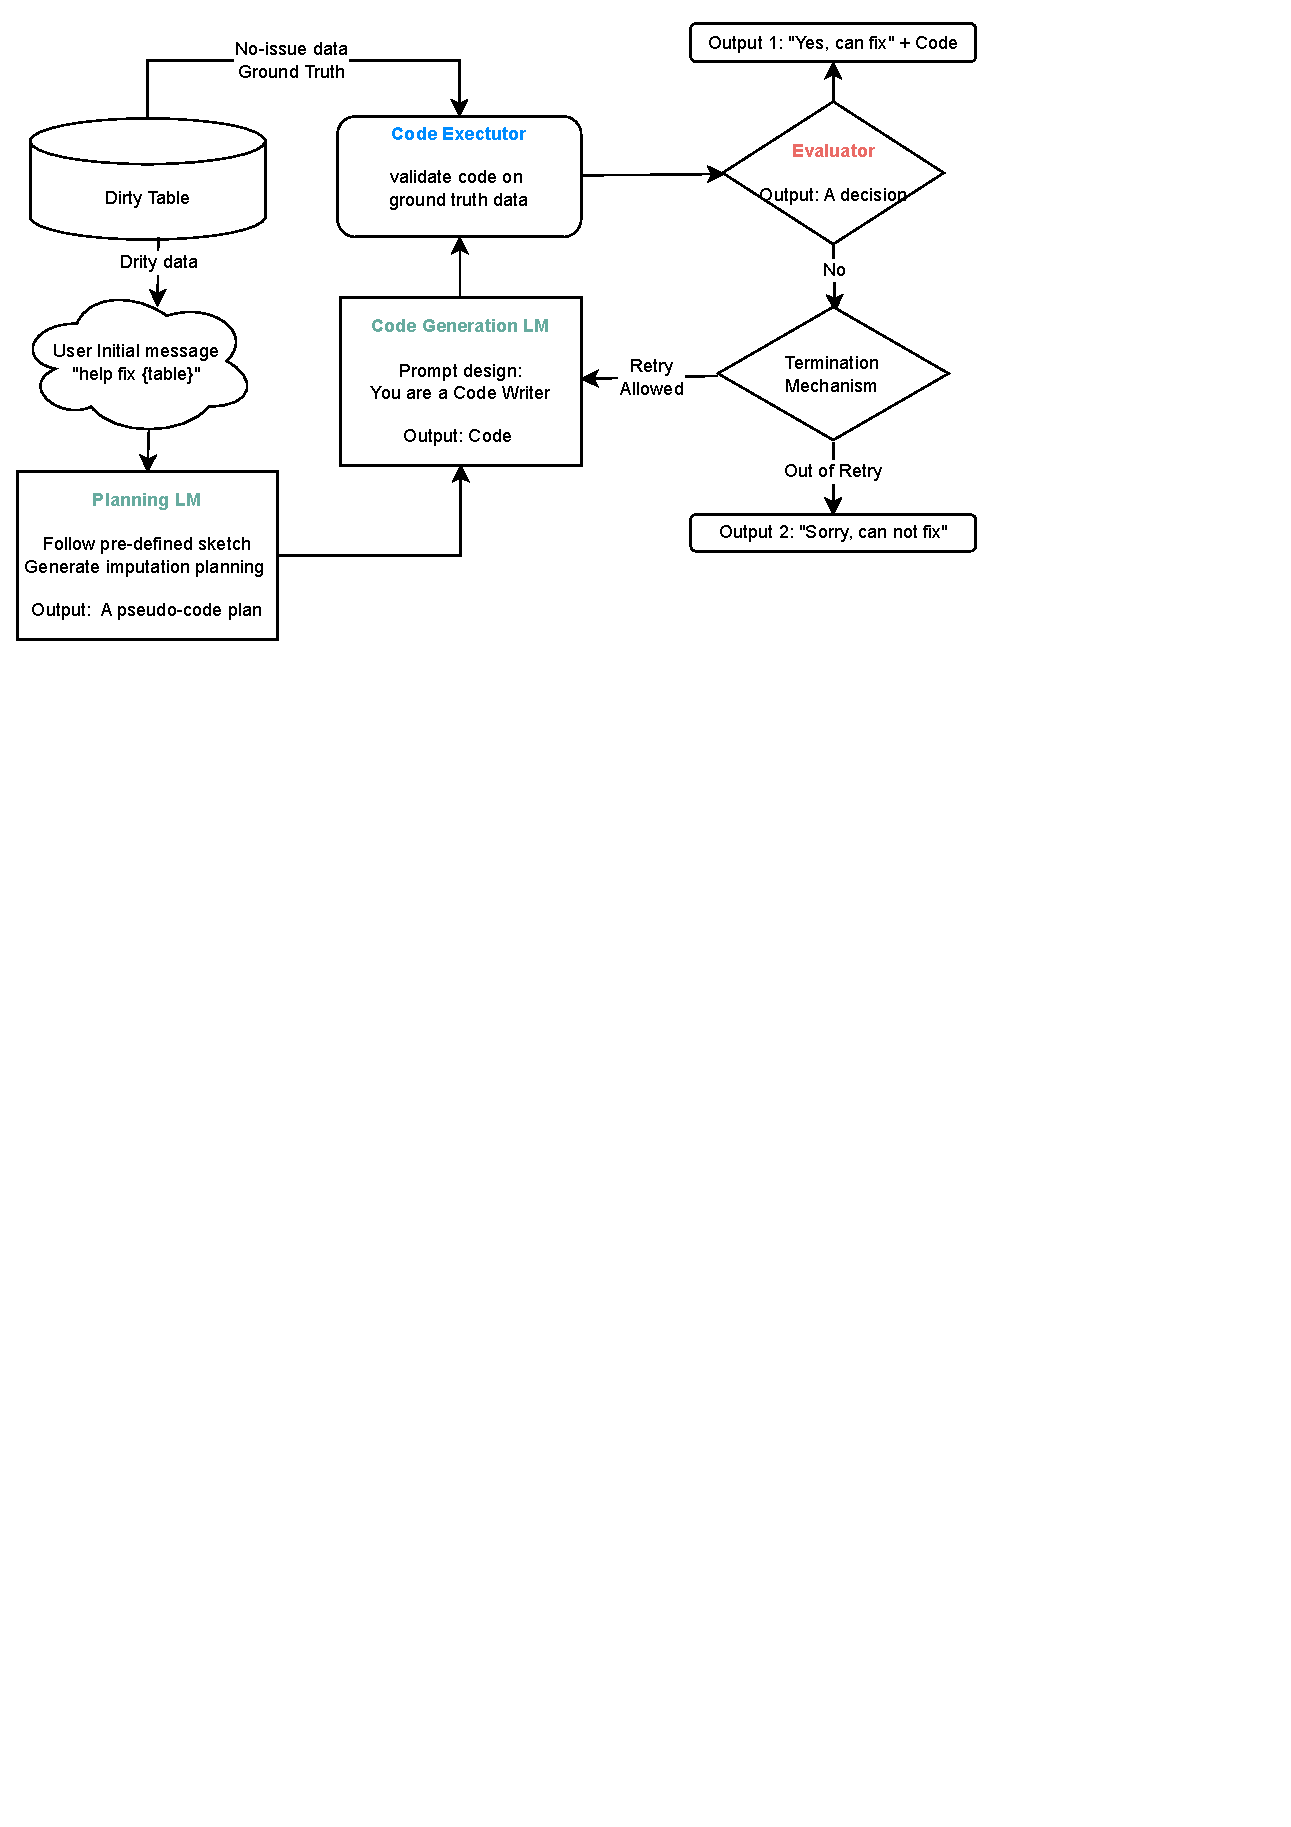
\includegraphics[width=\linewidth]{TabFill.pdf}
  \caption{An overview of TabFill}
  \label{fig:framework}
  % \description{haha}
\end{figure}


\subsection{Sketch-Guided Planning}
The sketch serves as a critical component in guiding the LLM for MVI tasks. Inspired by the instruction-following feature of LLMs~\cite{zhou2023instruction}, the sketch is predefined and specific to MVI on tabular data. It acts as a step-by-step instruction set for the LLM to plan the imputation steps. The predefined sketch in our later experiment includes: 1) identifying columns with missing values; 2) finding related columns that can help derive the missing values; 3) generating an imputation solution; 4) applying the solution; This structured approach leverages the domain knowledge embedded in LLMs, allowing for context-aware imputation strategies that outperform traditional methods.

\subsection{Code Generation}
As Inspired by previous research~\cite{poldrack2023ai}, the Code Generation LM bridges the gap between textual planning and code implementation. Given the importance of efficiency in MVI, converting imputation plans into executable scripts is a strategic choice. In our experiment, Python code is used to implement the MVI solutions, ensuring that the imputation process is not only automated but also easily verifiable and modifiable. This step enhances the transparency and portability of the imputation outcomes.

\subsection{Evaluator}
The evaluator acts as a decision-maker, crucial for validating the imputation results. It compares the executed output with ground truth data to assess the correctness of the current coding solution. If discrepancies are found, the system allows for retries to refine the code. This iterative validation process ensures high accuracy and reliability in the final imputed data.

Overall, TabFill’s innovative framework provides a robust, automated approach to MVI, leveraging the strengths of LLMs to deliver reliable and efficient solutions that significantly reduce the need for manual intervention.

\section{Experiment}

\subsection{Setup}

\paragraph{Approaches.} 
We compared TabFill with the following approaches:
(1) {\em LLM:} It utilizes LLM intuitively without any instructions.
(2) {\em CoT:} It prompts LLM to reply with ``Let’s think step by step''.

\paragraph{Backend LLM.}
We employ OpenAI's latest model, GPT-4-Turbo,\footnote{The newer model, gpt-4o was not released yet at the time of experiment} as the backend model. The GPT request is supported by API service from the Internet. The token size is set as 4096 using a temperature of 0. Specific to planning and Code LLM, they are both initialized by prompting techniques. In order to develop a Python executable runtime, we adopted the AutoGen framework~\cite{wu2023autogen}, which builds an interactive environment for agentic LLM. The code writer and code executor will complete the MVI job in automatic manner given a maximum retry limits.

\paragraph{Evaluation Metric.}
We assess overall accuracy by comparing imputed values to ground truth values using the exact match technique, and then counting the entire amount.

\subsection{Dataset}
In our experiments, we utilized two reprentative datasets from Kaggle to evaluate the performance of TabFill:

\begin{table}[h]
  \caption{Fact of dataset}
  \label{tab:dataset}
  \begin{tabular}{@{}lll@{}}
    \toprule
    Dataset              & Flight               & Supermarket    \\ \midrule
    \# of attributes     & 9                    & 6              \\
    \# of tuples per col & 5                    & 5              \\ 
    Testing variables      & Source, Total\_Stops & Tax 5\%, Total \\ \bottomrule
  \end{tabular}
\end{table}

\paragraph{Flight Price Prediction Dataset (Flight):} This dataset covers the historical airline flight of India during a certain period. It includes features such as source, destination, route, departure and arrival times, duration, and total stops. The dataset is used to predict flight prices based on these features. It offers a rich set of attributes with potential missing values that require imputation for accurate predictive modeling. In this dataset, we aim to backfill the Source and Total\_Stops fields (See Appendix~\ref{appendix:flight}). Based on the context information, we can conclude the relationship as below:
\begin{itemize}
  \item Source is equivalent to the first stop of Route, where the stop code should be translated to city name. Let us use Route: MAA → CCU for instance, the missing value of Source is translated from "MAA", which is Chennai.
  \item  Total\_Stops is equal to the number of arrows in Route, then minus one. For example, the missing value should be "1 stop" for the Route: DEL → HYD → COK.
\end{itemize}

\paragraph{Supermarket Sales Dataset (Supermarket):} The dataset is originally sourced from the 3-month historical sales transaction of a supermarket company in Myanmar. It includes features such as unit price, quantity, tax, total, and payment. The dataset is used to analyze and predict sales performance, requiring imputation of missing values to ensure comprehensive and accurate analysis. In this dataset, we aim to backfill the Tax 5\% and Total fields (See Appendix~\ref{appendix:supermarket}). Based on the context information, we can conclude the relationship as below:
\begin{itemize}
  \item $Tax\ 5\% = 5\% * (Unit\ price * Quantity)$, the special percentage in column name indicates the tax rate, thus, the missing value at the row 1 should be 33.25.
  \item $Total = (Unit\ price * Quantity) + Tax\ 5$, the total spending is tax included, thus, the missing value in row 4 is 19.95.
\end{itemize}

Notably, the \emph{Flight} dataset stands for logical-based associations between attributes. While, the \emph{Supermarket} dataset stands for formula-based associations.


\paragraph{Preprocessing.}
Each dataset is randomly segmented into subsets to accommodate the imputation of missing values that require proper strategies. Given the transparent association of the target variable to be imputed and other known variables, the subset is well curated as a testing tuple. Specifically, we mask the original values of the target variable with {\tt NaN} to mimic the missing value. We run a few experiments for demonstration purpose only. Full statistics are shown in Table~\ref{tab:dataset}.


\subsection{Result Analysis}
In this section, we report the performance of MVI using different approaches on two datasets. Please refer to the Table~\ref{tab:result}. Next, we will analyze the experimental results by dataset.

% \usepackage{booktabs}
\begin{table}[h]
  \caption{Experiment result using different approaches}
  \label{tab:result}
  \begin{tabular}{@{}lllll@{}}
    \toprule
                      & \multicolumn{2}{l}{Flight} & \multicolumn{2}{l}{Supermarket} \\ \midrule
    \textbf{Approach} & Source      & Total\_Stops & Tax 5\%        & Total          \\ \midrule
    LLM               & 3           & 3            & 5              & 5              \\
    CoT               & \textbf{4}  & \textbf{4}   & \textbf{5}     & \textbf{5}     \\
    TabFill           & \textbf{4}  & 2            & \textbf{5}     & 4              \\ \bottomrule
    \end{tabular}
\end{table}

\paragraph{Flight:}
\begin{itemize}
  \item LLM Approach: The basic LLM approach achieved a score of 3 for both the “Source” and “Total\_Stops” columns. This indicates a moderate level of accuracy but highlights potential limitations in handling more complex imputation tasks within the dataset.
  \item CoT Approach: This method shows an improvement over the basic LLM, achieving a score of 4 in both columns. The CoT approach benefits from its structured reasoning process, allowing for better context understanding and more accurate imputations.
  \item TabFill Approach: Our proposed TabFill framework matches the CoT approach in the “Source” column with a score of 4 but excels in the “Total\_Stops” column with a score of 2, indicating a lower accuracy. Because LLM may get confused by the representation learning of flight route, in particularly with symbols.
\end{itemize}

Below is a sample code snippet that TabFill generated eventually for MVI:
\begin{lstlisting}[language=Python, caption=Python function to impute missing values in Flight, label={code:flight}]
  # flight_2.py
  def impute_total_stops(route):
      stops_count = route.count('->') - 1
      if stops_count == 0:
          return 'non-stop'
      elif stops_count == 1:
          return '1 stop'
      elif stops_count == 2:
          return '2 stops'
      else:
          return f'{stops_count} stops'
  
  # flight_7.py
  def impute_missing_source(route):
      if route:
          return route.split("->")[0]
      return None
  
\end{lstlisting}
  
\paragraph{Supermarket:}
\begin{itemize}
  \item LLM Approach: The basic LLM approach performed consistently with scores of 5 in both the “Tax 5\%” and “Total” columns. This suggests challenges in achieving accurate imputations for the given attributes.
	\item CoT Approach: Similar to the LLM approach, the CoT method also scored 5 in both columns. While it improves reasoning, it did not significantly enhance the accuracy in this dataset.
	\item	TabFill Approach: TabFill maintained a perfect score of 5 for the “Tax 5\%” column, comparable to other methods, but demonstrated an improvement in the “Total” column with a score of 4. This improvement underscores TabFill’s ability to deliver more accurate and contextually aware imputations, facilitated by the structured output and validation mechanisms inherent in our framework.
\end{itemize}


Below is a sample code snippet that TabFill generated eventually for MVI:
\begin{lstlisting}[language=Python, caption=Python function to impute missing values in Supermarket, label={code:supermarket}]
  # supermarket_9.py
  def calculate_tax(unit_price, quantity):
      return (unit_price * quantity) * 0.05
    
  # supermarket_8.py
  def calculate_total(unit_price, quantity, tax):
      return (unit_price * quantity) + tax
\end{lstlisting}


Overall, TabFill exhibits a notable improvement in performance compared to other methods, particularly in the logical-associated columns where understanding the context is crucial. The integration of sketch-guided planning and code generation ensures that the imputation process is not only more accurate but also more efficient and scalable. This validation against ground truth data and iterative refinement further solidifies TabFill as a robust solution for missing value imputation in diverse datasets.


\section{Conclusion}
In this paper, we introduced TabFill, a novel framework for Missing Value Imputation (MVI) that leverages the capabilities of Large Language Models (LLMs) through a combination of sketch-based guidance, planning, and code generation. Our approach significantly enhances the efficiency of imputation tasks, reducing the reliance on manual intervention and providing a structured, executable output that is both transparent and flexible.

The results from our experiments on diverse datasets, including flight route and supermarket sales, demonstrate the effectiveness of TabFill. Our method not only outperforms traditional imputation techniques but also shows great performance compared to other LLM-based approaches. TabFill’s ability to generate context-aware imputations and convert them into verifiable Python code ensures robust and reliable data preprocessing.

Contributed to the framework design, the need for human input is minimized to the initial sketching and final code review stages, streamlining the MVI process. This approach not only reduces the time and effort typically spent on manual imputation but also mitigates the risk of human error. 


\section{Limitation}
While TabFill demonstrates significant improvements in Missing Value Imputation (MVI), it has certain limitations that need to be addressed in future work:
\begin{itemize}
  \item Dependency on Initial Sketch: The effectiveness of TabFill heavily relies on the quality and completeness of the initial sketch provided by the user. Inadequate or poorly defined sketches can lead to suboptimal imputation plans.
  
  \item Computational Cost: As API models are paid services, the computational cost associated with using LLMs can become a significant factor, especially for large-scale imputation tasks. This cost needs to be carefully managed and optimized to ensure the approach remains cost-effective.
  
  \item Handling Highly Correlated Missing Data: The current approach may struggle with datasets where missing values are highly correlated across multiple columns and rows, requiring more sophisticated techniques to accurately impute these values.
\end{itemize}

Future work will focus on refining the initial sketching process, exploring the use case for open-source model as backend, and validating across a wider array of datasets and domains. Additionally, integrating advanced techniques, such as LLM agent to handle highly correlated missing data will be a priority, aiming to further enhance the robustness and applicability of TabFill.


\bibliographystyle{ACM-Reference-Format}
\bibliography{report}


%% If your work has an appendix, this is the place to put it.

\newpage
\appendix


\begin{table*}[]
  \caption{Flight dirty demo}
  \label{appendix:flight}
  \centering
  \begin{tabular}{@{}llllll@{}}
  \toprule
  Airline     & Date\_of\_Journey & Source       & Destination & Route                 & Total\_Stops \\ \midrule
  IndiGo      & 12/06/2019        & Chennai      & Kolkata     & MAA → CCU             & non-stop     \\
  Jet Airways & 3/06/2019         & Mumbai       & Hyderabad   & BOM → HYD             & non-stop     \\
  Jet Airways & 15/06/2019        & Delhi        & Cochin      & DEL → LKO → BOM → COK & 2 stops      \\
  Jet Airways & 21/03/2019        & Delhi        & Cochin      & DEL → IXC → BOM → COK & 2 stops      \\
  Vistara     & 15/03/2019        & \textbf{NaN} & Kolkata     & MAA → CCU             & non-stop     \\
  IndiGo      & 3/03/2019         & Delhi        & Cochin      & DEL → HYD → COK       & \textbf{NaN} \\
  Air Asia    & 24/03/2019        & Kolkata      & Banglore    & CCU → DEL → BLR       & 1 stop       \\ \bottomrule
  \end{tabular}
\end{table*}

\begin{table*}[]
  \caption{Supermarket dirty demo}
  \label{appendix:supermarket}
  \begin{tabular}{@{}llllll@{}}
  \toprule
  Product line       & Unit price & Quantity & Tax 5\%      & Total        & Payment     \\ \midrule
  Home and lifestyle & 95         & 7        & \textbf{NaN} & 698.25       & Credit card \\
  Home and lifestyle & 24         & 7        & 8.4          & 176.4        & Ewallet     \\
  Home and lifestyle & 94         & 8        & 37.6         & 789.6        & Ewallet     \\
  Health and beauty  & 19         & 1        & 0.95         & \textbf{NaN} & Credit card \\
  Home and lifestyle & 49         & 10       & 24.5         & 514.5        & Credit card \\ \bottomrule
  \end{tabular}
\end{table*}

\end{document}
\endinput
%%
%% End of file `sample-sigconf-authordraft.tex'.
